\documentclass[11pt]{article}    	
\usepackage{geometry}      
\usepackage[latin1]{inputenc}  
\usepackage[T1]{fontenc}          		
\geometry{a4paper, margin=2.5cm} 
\usepackage{scrextend}  
\usepackage{tikz}
\usepackage{framed}
\usepackage{graphicx}
\usepackage{fancyhdr}
\usepackage{amsmath}

\newcommand\tab[1][1em]{\hspace*{#1}}


\pagestyle{fancy}
\rhead{Iacopo Sprenger 284074}
\lhead{Programmation I}
\setlength{\headheight}{14pt}
					
\begin{document}
\begin{center}
\Large \textbf{Projet d'Automne: Me too ?}
\end{center}
Une fois les param�tres entrez par l'utilisateur v�rifi�s, le programme commence les simulations. Le tout est structur� en trois boucles tout a l'ext�rieur il y a la boucle des contextes ensuite la boucle du taux de vaccination et finalement une boucle pour le nombre de simulations. 
\begin{figure}[htb]
\begin{framed}
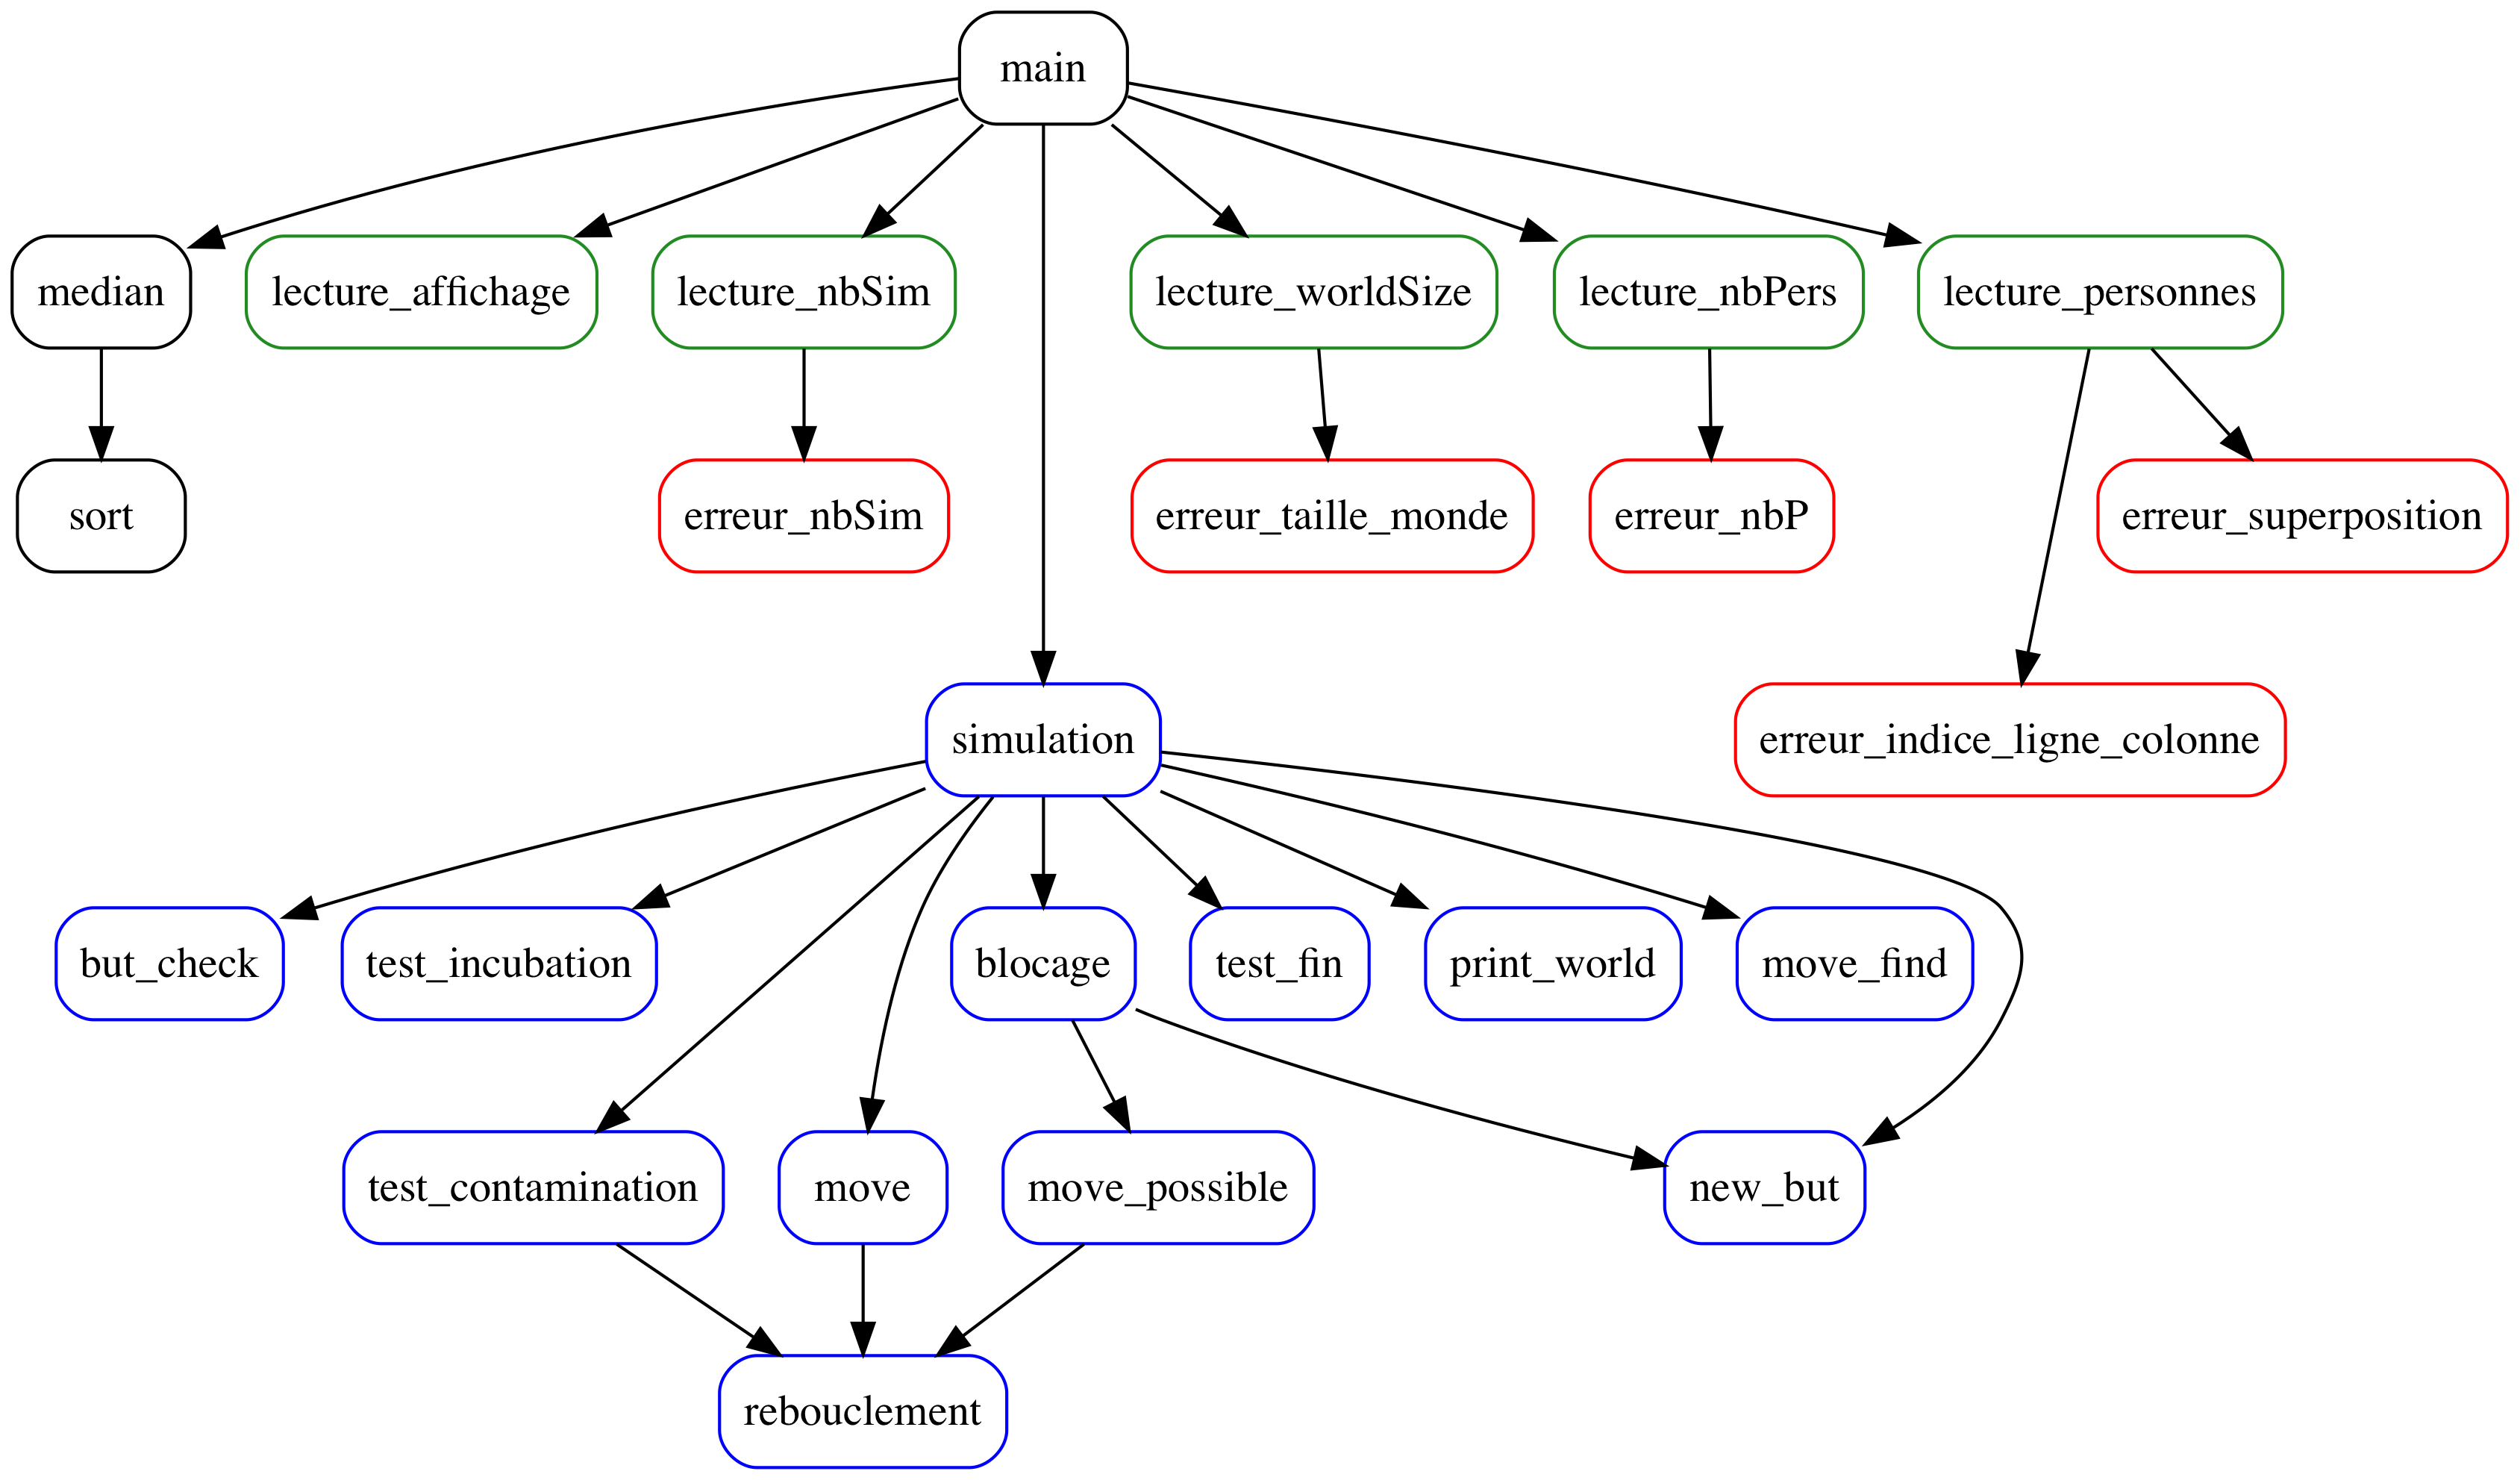
\includegraphics[scale=0.12]{graph.png}
\end{framed}
\caption{Diagramme des fonctions}
\end{figure}

\begin{figure}[htb]
\begin{framed} %pseudocode
\vspace{4pt}
1: \tab[0cm]\textit{simulations}[\textit{nbSim}]\\
2: \tab[0cm]\textbf{pour} \textit{contexte} \textbf{allant de} \textit{nbPers} \textbf{�} 1: \\
3: \tab[1cm]\textbf{pour} \textit{vaccination} \textbf{allant de} 0 \textbf{�} \textit{contexte}-1 : \\
4: \tab[2cm]\textbf{si} \textit{vaccination} est diff�rent de 0 : \\
5: \tab[3cm]\textit{people}[\textit{vaccination}][ETAT] $\leftarrow$ V \\
6: \tab[3cm]\textbf{pour} \textit{sim} \textbf{allant de} 0 \textbf{�} \textit{nbSim} : \\
7: \tab[4cm]\textit{simulations}[\textit{sim}] $\leftarrow$ \textbf{simulation}(contexte, vaccination, ...)\\
8: \tab[3cm]\textit{mediane} $\leftarrow$ \textbf{mediane}(\textit{simulations})\\
9: \tab[3cm]\textit{densit�} $\leftarrow$ \textit{$contexte/world\_size^2$}\\
10:\tab[3cm]\textit{taux\_vaccination} $\leftarrow$ \textit{$vaccination/contexte$}\\
11:\tab[3cm]\textbf{afficher} \textit{densit� \tab taux\_vaccination \tab mediane}\\
12:\tab[3cm]\textbf{pour} \textit{i} \textbf{allant de} 0 \textbf{�} \textit{contexte} - 1 : \\
13:\tab[4cm]\textit{people}[\textit{i}][ETAT] $\leftarrow$ N
\end{framed}
\caption{Pseudocode}
\end{figure}

\end{document} 











 